\documentclass[11pt, oneside]{article} 
\usepackage{geometry}
\geometry{letterpaper} 
\usepackage{graphicx}
	
\usepackage{amssymb}
\usepackage{amsmath}
\usepackage{parskip}
\usepackage{color}
\usepackage{hyperref}

\graphicspath{{/Users/telliott_admin/Tex/png/}}
% \begin{center} 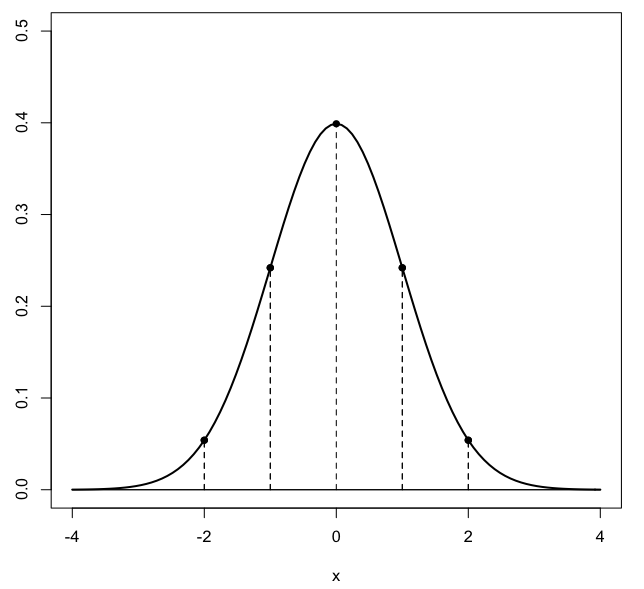
\includegraphics [scale=0.4] {gauss3.png} \end{center}

\title{Complex functions}
\date{}

\begin{document}
\maketitle
\Large
\subsection*{Complex numbers}

This will be a very brief introduction to a fairly difficult subject.  My hope is to make clear some elementary ideas about complex functions and the calculus of these functions, and to show their utility by computing one integral that we've already seen (for the normal distribution), that was a challenge using just the real numbers.

A complex number is simply an ordered pair $(x,y)$.  Typically, we label such numbers $z$ and write them as $z = x + iy$, where $i = \sqrt{-1}$.  By and large, this fact about $i$ isn't important.  What is important is that we have a rule for multiplication which says that

\[ z_1 \cdot z_2 = (x_1 + i y_1) \cdot (x_2 + i y_2) \]
\[ = \ [ x_1 x_2 - y_1 y_2 \ ] \ + i \ [ \ x_1 y_2 + x_2 y_1 \ ] \]
Using $i$ makes clear why $(iy)^2 = -y^2$.

\subsection*{Geometric interpretation}
Yet another powerful way to think about complex numbers is to use the complex plane (sometimes called the Argand plane), where points are plotted with the real part along the horizontal axis and the imaginary part along the vertical axis.

This figure is from Brown \& Churchill.
\begin{center} 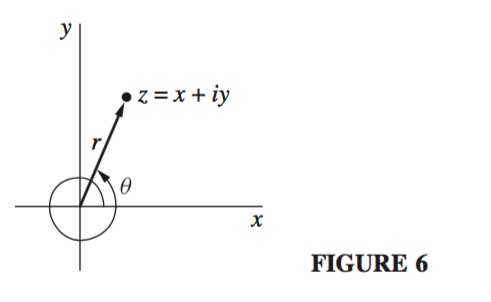
\includegraphics [scale=0.6] {Brown6.png} \end{center}

Looking at the graph, the distance of any point from the origin is denoted by $r$, and $\theta$ is the angle the ray makes with the positive $x$-axis in a CCW direction.  This should be familiar from standard polar coordinates.  Switching notation to
\[ z = x + iy \]
To plot the complex number $z$ we go out $x$ units along the real (horizontal) axis and then up $y$ units along the imaginary (vertical) axis.

The statement that $\mathbb{R} \subset \mathbb{C}$ is equivalent to the observation that the Argand plane contains the horizontal axis.  Real numbers have the form $z = x + i \cdot 0 = x$.

More generally, though
\[ x = r \cos \theta \]
\[ y = r \sin \theta \]
and
\[ x + iy = r \cos \theta + ir \sin \theta\]
\[ = r(\cos \theta + i \sin \theta) \]
\[ = re^{i\theta} \]
where the last part makes use of Euler's famous equation.  $r$ is called the \textbf{modulus} and $\theta$ is called the \textbf{argument} or \textbf{phase}.

Calculations are often easier using one form rather than another.  Here is multiplication in polar coordinates
\[ r e^{i\theta} \ \rho e^{i\phi} = r \rho \ e^{i (\theta + \phi)} \]
We multiply the distances and add the angles.  Here is the square function:
\[ (r e^{i\theta})^2 = r^2 e^{i2\theta} \]

\subsection*{Functions and derivatives}
A complex function is a function that takes a complex input $z$ and produces a complex output $w$, where
\[ w = u(x,y) + iv(x,y) \]
where $u$ and $v$ are real functions over $\mathbb{R}^2$.

If you think about differences between real and complex numbers, one big one is that for real numbers we are following a curve, and when we calculate the derivate at a point, there are only two directions from which to approach it.  For the complex plane, we can approach from atny direction in the plane.  It turns out that "good" functions, what are called \emph{analytic} functions, have the property that we can compute the derivative in a familiar way and obtain the same result in any direction.

An equivalent statement is that analytic functions obey the Cauchy-Riemann equations (CRE).
\[ u_x = v_y \]
\[ u_y = - v_x \]

It turns out that many familiar looking functions are analytic
\[ w = z^n \]
\[ w = e^z \]
\[ w = \sin z \]
\[ w = \cos z \]
while others are not.  Write
\[ z^2 = (x + iy)(x + iy) = x^2 - y^2 + i2xy \]
The above function is analytic, however
\[ (x - iy)(x - iy) = x^2 + y^2 - i2xy \]
is not, as one example.  It is not important to work out right now why it fails the CRE test.

\subsection*{Cauchy 1}

Cauchy's first theorem says that the integral of an analytic function over a closed path is equal to zero, when the enclosed region does not contain a singularity.
\[ \oint_C f(z) \ dz = 0 \]

This turns out to be a consequence of Green's Theorem, which you should remember from multivariable calculus.  Let
\[ z = x + i y \]
\[ dz = dx + i dy \]
\[ z = f(x,y) = u(x,y) + iv(x,y) \]
Our integral is
\[ \oint z \ dz = \oint (u(x,y) + iv(x,y)) \ (dx + i dy) \]
\[ =  \oint u(x,y) \ dx - \oint v(x,y) \ dy + i \oint v(x,y) \ dx + i \oint u(x,y) \ dy \]

As before, because we are moving along a curve there is a relationship between $x$ and $y$, so we can either express that relationship (for say, $y$ in terms of $x$), or parametrize the curve in terms of $t$ or $\theta$.  In either case, these become integrals in a single variable.  We suppress the $(x,y)$ notation and the extra integral signs:
\[ =  \oint u \ dx - v \ dy + i v \ dx + i u \ dy \]

\subsection*{proof of Cauchy 1}
Back in vector calculus we proved Green's theorem, which says that for two real functions of $x$ and $y$:  $M(x,y)$ and $N(x,y)$:
\[ \oint_C M dx + N dy = \iint_R (\frac{\partial N}{\partial x} - \frac{\partial M}{\partial y}) \ dx \ dy \]
Back then, $M$ and $N$ were components of a vector field $\mathbf{F}$ and we wrote the shorthand for curl:
\[ = \iint_R \nabla \times \mathbf{F} \ dA\]
but the important thing is that they are real-valued functions of two real variables $f: \mathbb{R}^2 \rightarrow \mathbb{R}^1$.

In terms of $u$ and $v$ we have for the real part of Cauchy's Theorem that $M=u$ and $N = -v$ (notice the minus sign!).  

So:
\[ \oint u \ dx - v \ dy = \iint_R (-\frac{\partial v}{\partial x} -  \frac{\partial u}{\partial y}) \ dx \ dy \]
\[ = - \iint_R (v_x + u_y) \ dx \ dy \]
But, according to the CRE
\[ u_y = -v_x \]
Hence, this integral is zero.

For the imaginary part we use Green's Theorem again with $N=u$ and $M = v$ (no minus sign here):
\[ \oint v \ dx + u \ dy =  \iint_R (\frac{\partial u}{\partial x} - \frac{\partial v}{\partial y}) \ dx \ dy \]
\[ =  \iint_R (u_x - v_y) \ dx \ dy \]
But, again, according to the CRE
\[ u_x = v_y \]
So the integral for the imaginary part is also zero, and thus the whole thing is zero as well:
\[ \oint u \ dx - \oint v \ dy + i \oint v \ dx + i \oint u \ dy = 0 \]

Remember how important it was (for Green's theorem) that the function being integrated be defined everywhere in the region.  Well, it's true here as well.

\[ \oint_C \frac{1}{z} \ dz \stackrel{?}{=} 0 \]

[in progress ]
We've already seen by direct calculation that this integral is \emph{not} zero when the curve $C$ includes the origin, but it \emph{is} zero otherwise.

\subsection*{example}

\[ f(z) = e^{-z^2} \]
Since
\[ z^2 = (x + iy)(x + iy) \]
\[ = x^2 - y^2 + 2ixy \]
We have
\[ f(z) = e^{-z^2} = e^{-x^2 + y^2 - 2ixy} \]
\[ = e^{y^2 - x^2} \ e^{i(-2xy)} \]
\[ = e^{y^2 - x^2} \ [ \ \cos -2xy + i \sin -2xy \ ] \]
\[ = e^{y^2 - x^2} \ [ \ \cos 2xy - i \sin 2xy \ ] \]
\[ = e^{y^2 - x^2} \cos 2xy - i e^{y^2 - x^2} \sin 2xy \]

Checking the CRE is a bit complicated:
\[ u = e^{y^2 - x^2} \cos 2xy \]
\[ u_x = (-2x) \  e^{y^2 - x^2} \cos 2xy -  2y \ e^{y^2 - x^2} \sin 2xy \]
\[ u_y = 2y \ e^{y^2 - x^2} \cos 2xy - 2x \ e^{y^2 - x^2} \sin 2xy \]
and
\[ v = - \ [ \ e^{y^2 - x^2} \sin 2xy \ ]  \]
\[ v_x = - \ [ \ -2x \ e^{y^2 + x^2} \sin 2xy - 2y \  e^{y^2 - x^2} \cos 2xy  \ ] \]
\[ v_y = - \ [ \ 2y \ e^{y^2 - x^2} \sin 2xy - 2x \ e^{y^2 - x^2} \cos 2xy \ ]  \]
Looks like a match.  $u_x = v_y$ and $u_y = - v_x$.

There is an important theorem that says that an analytic function $e^{w}$ of an analytic function $w = -z^2$, is itself an analytic function.  Since we won't prove this, I thought it better to check that the CRE are satisfied.

The next step Nahin carries out is to integrate this function around a particular contour:
\[ \int (u + iv) (dx + idy) \]
\[ = \int \{ u \ dx - v \ dy + i (u \ dy + v \ dx) \} \]

The path is rectangular
\begin{center} 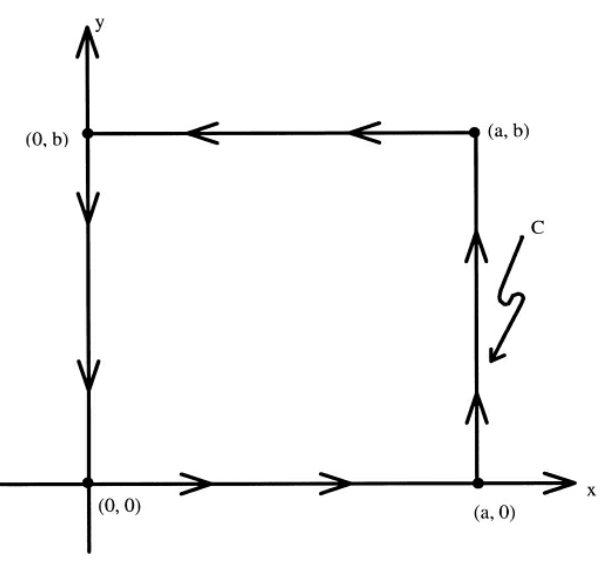
\includegraphics [scale=0.3] {nahin_path1.png} \end{center}

Cauchy does this integral at the beginning of his first, 1814, paper about complex functions.  He knows that the integral is zero due to the famous theorem we sketched above, Cauchy 1, since the function is analytic and does not blow up anywhere within the contour).

This means that both the real part and the imaginary part must be equal to zero.

We have four different parts with four different paths.  To keep this simpler, I will only do the real part.

Part 1:  $(0,0) \rightarrow (a,0)$
\[ I_1 = \int  u \ dx - \int v \ dy \]
$dy = 0$ so
\[ I_1 = \int u \ dx \]
\[ = \int_0^a e^{y^2 - x^2} \cos 2xy \ dx \]
$y = 0$ so
\[ I_1 = \int_0^a e^{- x^2} \cos 0 \ dx \]
\[ = \int_0^a e^{- x^2} \ dx  \]

Part 2: $(a,0) \rightarrow (a,b)$
\[ I_2 = \int  u \ dx - \int v \ dy \]
$dx = 0$ so
\[ I_2 = - \int_0^b v \ dy \]
\[ = - \int_0^b e^{y^2 - x^2} \sin 2xy \ dy \]
$x = a$ so
\[ I_2 = - \int_0^b e^{y^2 - a^2} \sin 2ay \ dy \]
\[ = - e^{- a^2} \int_0^b e^{y^2} \sin 2ay \ dy \]

Part 3:  $(a,b) \rightarrow (0,b)$
\[ I_3 = \int  u \ dx - \int v \ dy \]
$dy = 0$ so
\[ I_3 = \int_a^0 e^{y^2 - x^2} \cos 2xy \ dx  \]
$y = b$ so
\[ I_3 = \int_a^0 e^{b^2} \ e^{- x^2} \cos 2xb \ dx  \]
\[ = - e^{b^2} \int_0^a e^{- x^2} \cos 2xb \ dx  \]

Part 4: $(0,b) to (0,0)$
\[ I_4 = \int  u \ dx - \int v \ dy \]
$dx = 0$ so
\[ I_4 = \int - v \ dy \]
\[ = \int_b^0 e^{y^2 - x^2} \sin 2xy \ dy \]
$x = 0$ so
\[ I_4 = 0 \]

Adding together

\[ 0 =  \int_0^a e^{- x^2} \ dx - e^{- a^2} \int_0^b e^{y^2} \sin 2ay \ dy  - e^{b^2} \int_0^a e^{- x^2} \cos 2xb \ dx \]
\[  \int_0^a e^{- x^2} \ dx = e^{- a^2} \int_0^b e^{y^2} \sin 2ay \ dy  + e^{b^2} \int_0^a e^{- x^2} \cos 2xb \ dx \]

Does that look like progress?

Now, let $a \rightarrow \infty$ !!  The first term on the right-hand side goes to zero because $e^{-a^2} \rightarrow 0$ so
\[ \int_0^{\infty} e^{- x^2} \ dx = e^{-b^2} \int_0^{\infty} e^{- x^2} \cos 2xb \ dx  \]

We were supposed to already do the right-hand integral.
\[ \int_0^{\infty} e^{- x^2} \cos 2xb \ dx = \frac{\sqrt{\pi}}{2} \]

Hence:
\[ e^{-b^2}  \int_0^{\infty} e^{- x^2} \ \cos 2bx \  dx = e^{-b^2}  \ \frac{\sqrt{\pi}}{2} \]
when $b = 0$
\[ \int_0^{\infty} e^{- x^2} \  dx = \frac{\sqrt{\pi}}{2} \]




\end{document}